
% ****** Start of file apssamp.tex ******
%
%   This file is part of the APS files in the REVTeX 4.1 distribution.
%   Version 4.1r of REVTeX, August 2010
%
%   Copyright (c) 2009, 2010 The American Physical Society.
%
%   See the REVTeX 4 README file for restrictions and more information.
%
% TeX'ing this file requires that you have AMS-LaTeX 2.0 installed
% as well as the rest of the prerequisites for REVTeX 4.1
%
% See the REVTeX 4 README file
% It also requires running BibTeX. The commands are as follows:
%
%  1)  latex apssamp.tex
%  2)  bibtex apssamp
%  3)  latex apssamp.tex
%  4)  latex apssamp.tex
%
\documentclass[%
 reprint,
%superscriptaddress,
%groupedaddress,
%unsortedaddress,
%runinaddress,
%frontmatterverbose, 
%preprint,
showpacs,
%preprintnumbers,
%nofootinbib,
%nobibnotes,
%bibnotes,
 amsmath,amssymb,
 aps,
%pra,
%prb,
%rmp,
%prstab,
%prstper,
%floatfix,
longbibliography,
]{revtex4-1}

\usepackage{graphicx}% Include figure files
\usepackage{dcolumn}% Align table columns on decimal point
\usepackage{multirow}
\usepackage{bm}% bold math
\usepackage{hyperref}% add hypertext capabilities
\usepackage[mathlines]{lineno}% Enable numbering of text and display math
%\linenumbers\relax % Commence numbering lines

%\usepackage[showframe,%Uncomment any one of the following lines to test 
%%scale=0.7, marginratio={1:1, 2:3}, ignoreall,% default settings
%%text={7in,10in},centering,
%%margin=1.5in,
%%total={6.5in,8.75in}, top=1.2in, left=0.9in, includefoot,
%%height=10in,a5paper,hmargin={3cm,0.8in},
%]{geometry}

\begin{document}

\preprint{qoqp}

\title{Superconducting Qubits}% Force line breaks with \\
%\thanks{A footnote to the article title}%

% All people from 1st institution
\author{Joseph Camilleri}
%\homepage{http://www.first.institution.edu/~Charlie.Author}
%\altaffiliation[Also at ]{Physics Department, XYZ University.}%Lines break automatically or can be forced with \\
\affiliation{Physics Department, Virginia Tech}%
%\collaboration{SuperCDMS}%\noaffiliation

%
%\collaboration{SuperCDMS}%\noaffiliation

\date{\today}% It is always \today, today,
             %  but any date may be explicitly specified

\begin{abstract}

Superconducting resonators coupled to Josephson junctions (superconducting qubits) provide a platform for quantum computation. Of practical importance, they also present a tractable recipe to systematically fabricate and scale a system of controllable and addressable qubits. In addition to being a means to realize quantum algorithms, the development of superconducting qubits the past two decades has required the analysis of physical problems that have proven to be interesting in their own right. Numerous methods for realizing quantum-coherent states have been researched, with the transmon qubit garnering popularity because of its utility in decoupling ubiquitous charge noise present in solid state systems. We will explore the development of superconducting qubit technology, discuss dielectric loss in two-level systems (TLS) and how it has shaped the development of qubits, and also offer a view on the outlook of future systems.

\end{abstract}


%\pacs{29.40.Wk, 95.55.Vj, 95.35.+d}% PACS, the Physics and Astronomy
                             				% Classification Scheme.
%\keywords{Suggested keywords}%Use showkeys class option if keyword
                              %display desired
\maketitle

%\tableofcontents
\section{introduction}
The exploration of superconductivity as a fundamental phenomena in tandem with the engineering of technologies leveraging its striking features has grown into a rich discourse between theory and experiment the past century. Often, to further study physics, sensitive and precise devices are required that in turn demand a new understanding of physics. Some examples of such devices include: transition-edge sensors (TES) that leverage the sharp superconducting transition for calorimetry \cite{Irwin_TES}, microwave kinetic inductance detectors (MKIDs) that image photons from the cosmos via the kinetic induction's dependence on quasiparticle density \cite{mkidjpl}, and Josephson junctions that manifest quantum coherent states as charge or flux eigenstates of a superconducting qubit \ \cite{Clarke}.

The basis for storing quantum information in superconducting qubits starts with the idea of macroscopic quantum coherence, suggested by Leggett during the 1980's \cite{Leggett}. The main idea is that certain variables of Bose-Einstein condensate-like states associated with superfluids and superconductors form macroscopic quantities. Quantum mechanical tunneling between these macroscopic states allows for the creation of coherent-superposition states, which Leggett further suggested to be practically achieveable in superconducting quantum interference devices (SQUIDs). Some macroscopically observable quanta for such a system include the \textit{magnetic flux} \ (originating from the superconducting wavefunction phase \ \cite{josephson}) and the \textit{number of bound Cooper pairs} \ (originating from the electron-phonon interaction \ \cite{bcs}). The hope is that these quantities would be large enough and localized so that they can be studied more accessibly in experiment.

SQUIDs' interesting and useful physical properties arise from the quantum-interference pattern between the macroscopic wave functions of two superconductors, separated by an insulating layer (the Josephson junction \cite{josephson}). This system can be fabricated by depositing metallic thin-films onto a crystalline substrate, that are then interfaced together by an insulating metal-oxide. The dynamics of a current of Cooper pairs and the superconducting phase across a DC voltage-biased Josephson junction are goverened by two equations:

\begin{align*}
I &=I_o \textrm{sin}\left(\delta\right) \\
\hbar\dot{\delta} &= \hbar\omega = 2\textrm{eV}
\end{align*}

Where $\delta$ progresses linearly in time, $\omega=\dot{\delta}$ gives the frequency of oscillation of the superconducting current, and $I_o$ is the critical current of the Josephson junction. This "AC-Josephson Effect" also works in reverse: if the phase in the circuit changes over time, this induces sinusoidal current oscillations and a DC voltage across the junction. This two-terminal circuit is known as the RF-SQUID \cite{squid} and forms the core of many superconducting qubit platforms.

Using these two equations, we see that the junction forms a non-linear inductance where it can store magnetic potential energy.

\begin{align*}
L_J &= \phi_o / \left(2\pi I_o cos(\delta)\right) \\
U_J &= \frac{I_o\phi_o}{2\pi} cos(\delta)
\end{align*} It also follows that upon comparison with Faraday's law, the superconducting phase is related to the induced magnetic flux in the current loop, which is quantized in units of the magnetic flux quanta, $\phi_o$.

\begin{align*}
\delta &= \Phi \cdot 2\pi / \phi_o \\
\phi_o &= h/2e
\end{align*}

The number of Cooper pairs on the junction terminal, along with the superconducting phase across it, constitute a set of canonically conjugate operators that describe the energy of the system.
\begin{equation*}
\left[\hat{\delta},\hat{n}\right] = -i
\end{equation*}
In other words, they obey the generalized Heisenberg uncertainty relation. As a consequence, we will see in different superconducting qubit circuits the phase and Cooper pair number exchange roles as the localized quantum variable of the system where we store information.

\section{implementations}
The first superconducting qubit platform to demonstrate macroscopic quantum coherence was the Cooper pair box in 1999 \cite{Nakamura_1999}, approximately 20 years after Leggett's initial proposition. This time difference speaks to the tremendous advances in fabrication technology required to realize superconducting qubits.  The Cooper pair box operates as the simplest possible charge based qubit. A gate capacitor couples an RF squid to an applied gate voltage. Given the capacitor is small, the charging energy of the circuit should be much larger than the thermal energy at a given temperature. The dispersion of flux will be large for a large charging energy relative to inductive energy, and the number of Cooper pairs is well localized. Therefore, we can define the computational basis for such a qubit as two adjacent number states.

\begin{align*}
|0\rangle &= |n\rangle \\
|1\rangle &= |n+1\rangle
\end{align*}

The Hamiltonian for a general charge qubit involves energy stored in magnetic and electric fields :

\begin{equation*}
H = 4E_C (\hat{n}-n_g)^2 - E_J \textrm{cos}(\hat{\delta})
\end{equation*}

Where  $E_C = (2e)^2/C$ is the capacitor charging energy and $E_J=I_o\phi_o /(2\pi)$ is the Josephson energy of the inductance.
While the charging energy should dominate dynamics, the Josephson energy is essential to allow tunneling between charge states and provide an anharmonic spectrum.
\begin{figure}[h!]
  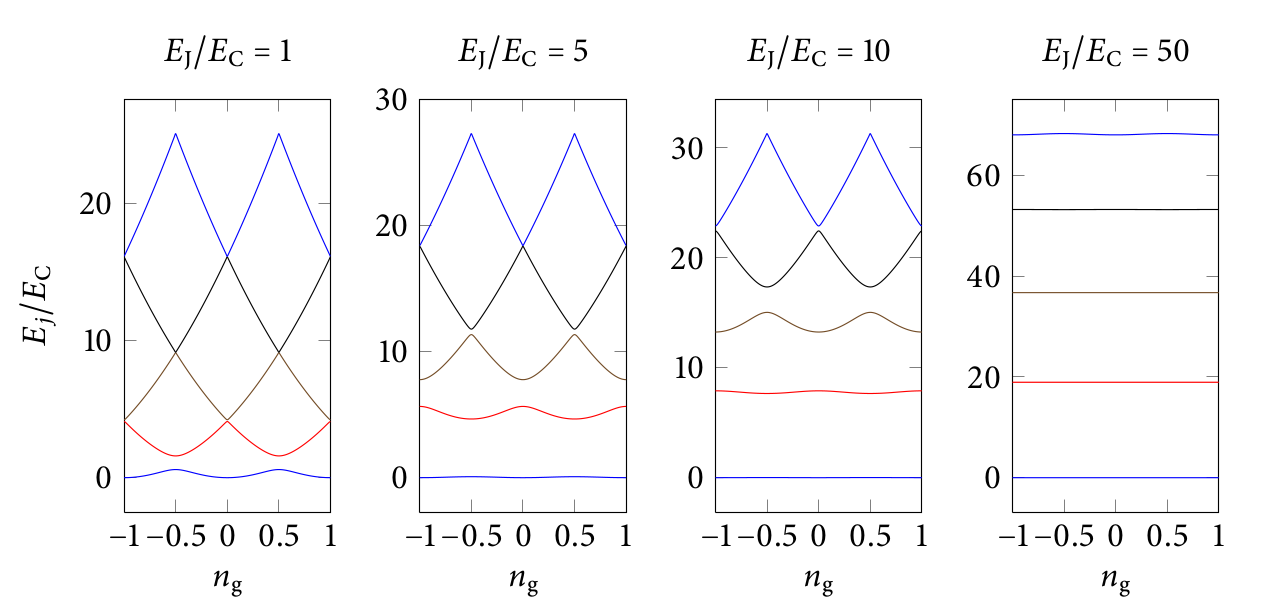
\includegraphics[width=\linewidth]{charge_dispersion_full.png}
  \caption{Plot of energy levels normalized to the charging energy versus the applied gate charge. As we increase $E_J/E_C$ there is both reduced charge dispersion and anharmonicity. Simulation data taken from \ \cite{bishop}}
  \label{fig:cd}
\end{figure}

Observing the change in energy with respect to gate charge (Fig. \ \ref{fig:cd}) gives a concise explanation for the adoption of the transmon qubit as the standard charge qubit platform. While the CPB regime (small $E_J/E_C$) displays superior anharmonicity, it is clear the qubit frequency is quadratically sensitive to perturbations in the gate charge. Charge noise, as we will see, is an imposing noise soure in superconducting qubits, so trading anharmonicity for charge noise suppression is a welcome compromise. In the regime $E_J/E_C \approx 50-100$, the eigenstates are no longer purely charge states (the Josephson energy contributes more to dynamics) but the spectrum is now far less sensitive to perturbations in the gate charge. 
\begin{figure}[h!]
  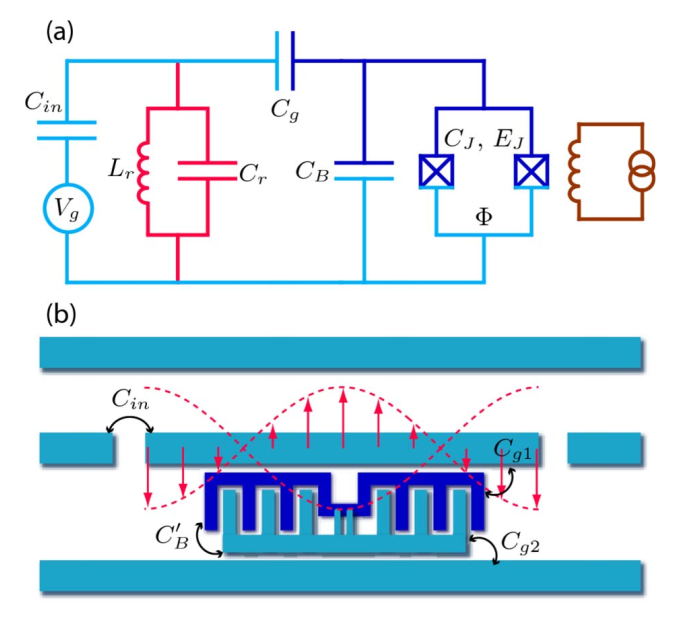
\includegraphics[width=\linewidth]{transmonfig.png}
  \caption{The transmon qubit. The resonator coupling replaces the DC voltage bias originally used to control the CPB and a shunting capacitance increases $E_J/E_C$. Illustration from the original paper proposing the transmon qubit architecture \cite{Transmon}.}
  \label{fig:transmon}
\end{figure}

The transmon qubit, illustrated in Fig. \ref{fig:transmon} was proposed in 2007 \cite{Transmon} to combat charge noise and would break the microsecond threshold for coherence times that was previously unnattainable in a platform that was also reproduceable. The transmon adds an additional capacitance in parallel with a DC SQUID \cite{squid} to decrease the charging energy and boost the ratio of $E_J/E_C$ while having a tuneable qubit frequency. It also utilizes a transmission line resonator coupling in place of a gate charge bias, which enables for microwave control of the device. The accumulation of charge on the island (and absence of charge on the opposite terminal) implements a natural dipole distribution of charge which seamlessly allows for coupling to the microwave field, as described in the Jaynes-Cummings model \ \cite{jaynescummings}. This naturally contrasts the flux qubit, which resembles a magnetic dipole and operates in a regime of localized flux states.

The first flux qubit was implemented several months after the Cooper pair box in 1999 \cite{fluxqubit}. Flux qubits can be implemented with a varying number of Josephson junctions in a given loop; we will discuss the three junction case. Two of the junctions are larger by a factor of $\gamma$ than the third junction. Each junction has its own phase that enters the Hamiltonian, however the phase quantization condition for the entire loop can be used to reduce the degrees of freedom to just the phases of the two larger junctions. When an external flux bias of $\phi_o /2$ threads the loop, known as the 'sweet spot' or 'flux insensitive bias', the Hamiltonian can be treated as a quasi-1D problem \cite{scqb_intro}.

\begin{equation*}
\hat{H} = 4E_C \hat{n}^2 - E_J \textrm{cos}(2\hat{\delta} + \phi_{external}) - 2\gamma E_J\textrm{cos}(\hat{\delta})
\end{equation*}

When biased at this point, the potential energy assumes a quartic shape, where the two minima correspond to anti-parallel flux states (equivalently clockwise/counter-clockwise supercurrents). The barrier height separating the two regions is shallow enough to permit significant tunneling, and the computational basis is formed by superpositions of the two flux states.

\begin{align*}
|0\rangle &= \frac{1}{\sqrt{2}}\left(|\uparrow\rangle +  |\downarrow\rangle\right) \\
|1\rangle &= \frac{1}{\sqrt{2}}\left(|\uparrow\rangle -  |\downarrow\rangle\right)
\end{align*}

\begin{figure}[h!]
  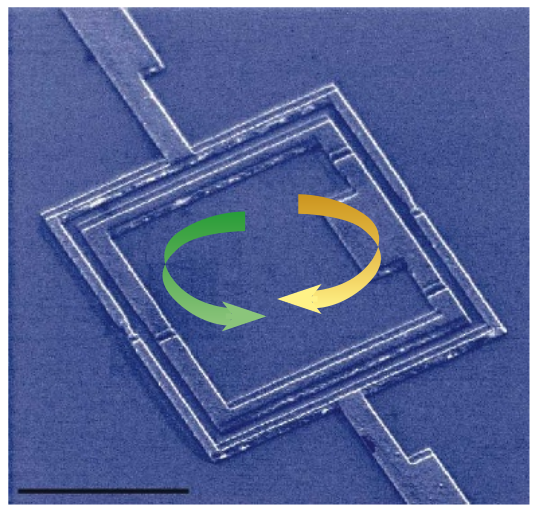
\includegraphics[width=\linewidth]{wilhelm_ckt.png}
  \caption{Original flux qubit architecture with three Joseph junctions connected in series to boost $E_J/E_C$. The two anti-parallel flux states are illustrated as circulating superconducting currents. Illustration from \cite{Wilhelm}.}
  \label{fig:fluxqubit}
\end{figure}
The advantage flux qubits natively have is that the energy spectrum is strongly anharmonic; in general 80 times greater than a typical transmon qubit \cite{birenbaum}. Then, if flux qubits are strongly anharmonic and operate in a regime less sensitive to charge noise, it begs the question why their development largely stalled for a decade despite demonstrating near microsecond coherence years before the transmon \cite{microsecond_fluxqubit}.

The issue stems from the inability to fabricate low dissipation inductors. To place the device firmly in the localized flux regime we require $E_J/E_C \gg 1$. However, the only way to make an extremely low-loss inductance is by adding more Josephson junctions to the loop. As will be discussed in the next section on dielectric loss, Josephson junctions need to be fabricated on the order of 10-100 square nanometers to have competitive coherence times. Device length scales of this order are not feasible using standard photolithographic techniques and thus require more complicated lithography, namely electron beam lithographic techniques. The practical consequence is that early flux qubits were difficult to reproduce reliably and performance heavily depended on the symmetry of the Josephson junctions\cite{birenbaum}, which we just argued are complicated to fabricate.

A third distinct superconducting circuit used to demonstrate quantum coherence is the phase qubit \cite{PhaseQubit}. The circuit consists of an RF-SQUID with a very large shunting capacitance. This is the same topology as the transmon, however the capacitor is so large ($E_J / E_C \approx 10^4-10^6$)  that the device operates far from the regime of charge being localized across the junction. We note that this large ratio of Josephson to charging energy is achieved differently than the flux qubit or fluxonium, where the inductance was boosted by increasing the number of junctions in the loop. The large Josephson energy allows macroscopic bias currents to flow through the junction which couple to the Hamiltonian's third term.

\begin{equation*}
H = 4E_c \hat{n}^2 -E_J \textrm{cos}(\hat{\delta}) -\frac{I \phi_o}{2\pi}\hat{\delta}
\end{equation*}

This allows the qubit transition frequency to be continuously tuned by the bias to the phase qubit. When biased near the critical current of the junction, the phase qubit forms a cubic potential \cite{Clarke}, where both minima serve different purposes for read out.

\begin{figure}[h!]
  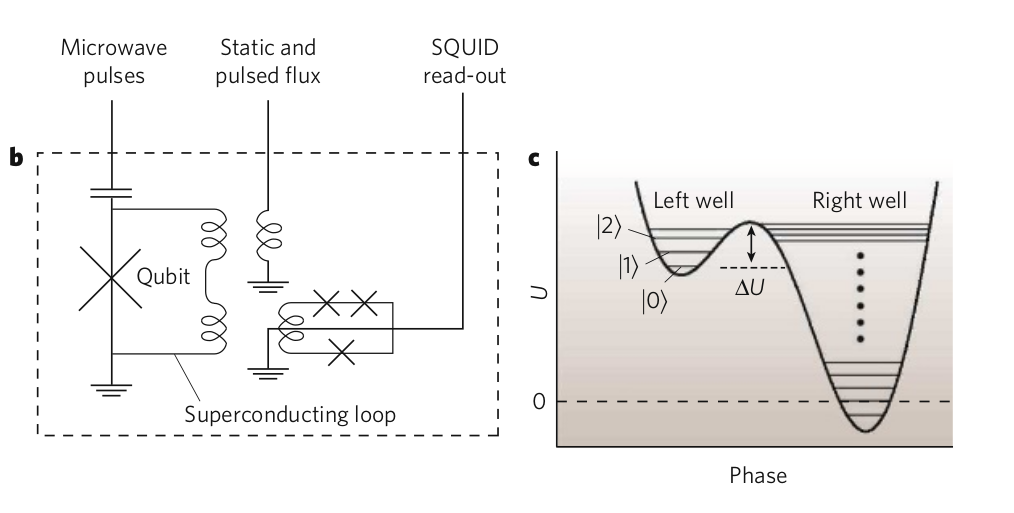
\includegraphics[width=\linewidth]{phase_qubit.png}
  \caption{Phase qubit potential energy profile and readout circuit. The flux state, from which tunneling is inferred from the second excited state, is read out through an inductively coupled DC squid. Current bias and microwave flux are both applied inductively through a second inductive coupling. Illustration from \cite{Clarke}.}
  \label{fig:phasequbit}
\end{figure}
 The shallow minimum contains a strongly anharmonic spectrum and encodes the computational basis $|0\rangle$ and $|1\rangle$. To readout the state, microwave energy corresponding to the transition from the second excited and first excited states is applied. If the qubit state $|1\rangle$ transitions to $|2\rangle$, there is a high probability of tunneling to the second potential energy minimum. The the final readout of the circuit involves measuring the flux, which directly tells the user which potential well the state resides in, and hence if tunneling has occured. This measurement setup is quite elegant, but strongly depends on the anharmonicity of the shallow well, and the shallowness of the barrier separating the two flux states. The phase qubit demonstrated first tomographic reconstruction of Bloch precession due to decoherence, a testament to the high measurement fidelity (for the time period) of 90$\%$ \cite{TLS_phasequbit}. 

It is further worth noting the phase qubit is distinct from flux qubits, although both operate with large ratios of $E_J/E_C$. The flux qubit explicitly encodes information in anti-parallel flux states. The phase qubit leverages flux to perform readout but the actual information is not encoded in complemetary magnetic dipole-like flux configurations. The historical irony with the phase qubit is that it was developed to combat ubiquitous charge noise that dominated decoherence in early charge qubits. However the use of a large \textit{dielectric} capacitor to mitigate charge noise would contribute to the discovery of the dominant mechanism underlying this noise source in superconducting qubits.

\section{dielectric loss and decoherence}
After the excitement of demonstrating macroscopic coherence using the Cooper pair box in 1999, growing experimental evidence pointed towards an unknown mechanism generating noise in charge qubits \ \cite{Astafiev_2004}. This noise attracted interest because of its large magnitude relative to other noise sources, the simultaneous observation of it in superconducting resonators used in astronomy \ \cite{zmuidzinas}, and  that it behaved in a complex manner. In particular, the noise displays a 1/f distribution at low frequencies manifesting as pure dephasing ($T_\phi$). At high frequency, frequency proportional noise contributes  to energy relaxation ($T_1$) and intersects the 1/f spectrum at a characeristic frequncy $\omega = T$ . In addition, the integrated noise power weighting the 1/f portion shows a $1/T^2$ dependence and the total noise power decreases with increasing microwave drive in the qubit. 

These combined features were irreconcilable with bosonic modes of dissipation (as used to describe photons and phonons). The same year as this noise study,  Makhlin et al. \cite{Mahklin_TLS} proposed a model suggesting a fermionic bath of two-level systems interact with the qubit and generate dissipation. Remarkably, this explanation managed to simulataneously describe all of the experimental features just mentioned. The following year (2005), Martinis et al. \cite{Martinis_2005} supplied strong experimental evidence to confirm this claim comparing data between phase qubits with two different junction areas (see Fig. \ref{fig:TLS}). They attributed the bath of TLS to microscopic defects in amorphous dielectric materials. Essentially, the random structure of the dielectric creates a potential energy landscape with many minima for atoms to tunnel between. The microwave electric field of the qubit easily couples to the dipole moments of each TLS and induces dissipation. Intuitively it can be viewed as the coupling of many 'tiny qubits' that remove information from qubit of interest, having a uniform distribution of energy splittings.

\begin{figure}[h!]
  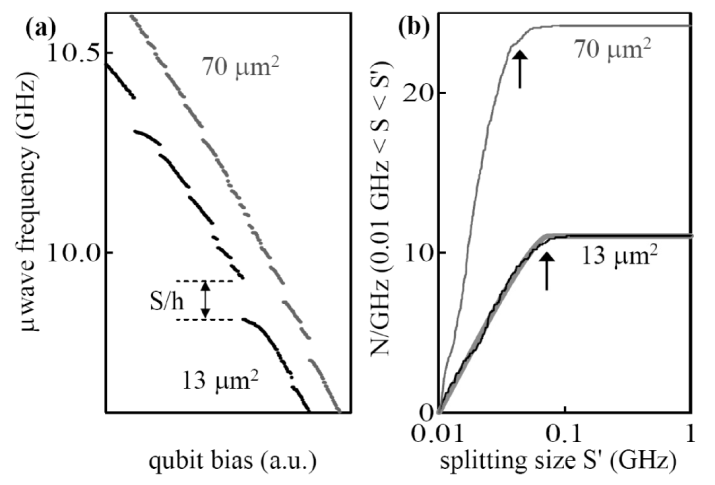
\includegraphics[width=\linewidth]{TLS.png}
  \caption{Experimental data from \cite{Martinis_2005} showing a uniform distribution of energy splittings (b) as predicted by the TLS model proposed by \cite{Mahklin_TLS}
  The dramatic effect of the resonant TLS coupling to the qubit frequency (a) is observed for two junctions with different area. The initial sloping region before the predicted uniform distribution is consistent with the TLS model and is an effect of the junction size.}
  \label{fig:TLS}
\end{figure}

This experimental study had significant implications for the next decade of superconducting qubit design. One such implication was how these defects scaled for differently sized Josephson junctions. For junctions larger than 10 square microns, the loss of the system is described by a continuum ensemble of TLS with uniform energy splittings. Quantitatively, the loss tangent captures the relative weight of dissipation and pure oscillation in the dielectric
\begin{equation*}
\delta = \frac{\textrm{Im}(\epsilon)}{\textrm{Re}(\epsilon)} = \frac{\pi(ed)^2 \rho}{3\epsilon}\frac{\textrm{tanh}(\hbar\omega/2k_B T)}{\sqrt{1+\omega_R T_1 T_2}}
\end{equation*}
where $\omega_R$ is the Rabi frequency of a TLS, $\rho$ is the density of states of the TLS, and $T_1$ and $T_2$ are the relaxation and dephasing coherence times of the TLS respectively. Below 1 square micron of junction size, the dielectric only couples a discrete 'sparse bath' of TLS. In general, these TLS are statistically avoided from coupling directly to the qubit frequency (the worst case scenario) but  still contribute to the overall broadband 1/f noise responsible for dephasing. The issue this implies is that for a future quantum computing platform with thousands or millions of qubits, the statistics of resonating the qubit with a TLS would be relevant in degrading $T_1$ times of a subset of a massive system.

A further more immediate impact of TLS noise is the fabrication methodology of superconducting qubits in general. TLS defects can manifest primarily in 3 places on a given chip: the Josephson junction insulating barrier, any dielectric based capacitor, and any interface of superconducting metal with the crystalline substrate. To mitigate losses, quality superconudcting films have been important for improved coherence, because of the large surface they occupy on a chip. In particular, the utilization of molecular beam epitaxy in depositing superconducting films was adopted from the field of astronomy (used in superconducting resonators previously mentioned in regards to TLS noise) to reduce lossy metal-substrate interfaces \cite{MBE}. Additionally, it was found in another 5-year study on dielectric loss \cite{UCSB2015_decoherence} that oxygen trapped during dielectric growth is strongly correlated with TLS defects. Thus, when a dielectric is necessary in a superconducting qubit circuit, the choice of dielectric material in hand with the method it is grown are very important.

Lastly, to improve coherence times without changing a given fabrication material, chips are often designed with 'participation ratios' in mind.
In the context of TLS noise, the participation ratio refers to the amount of dielectric interface on a given chip that is exposed to microwave fields, and can therefore couple to the qubit. Two designs that reflect innovative engineering to minimize participation ratios are the xmon qubit\cite{xmon} and the 3D transmon\cite{3dtransmon}.

The xmon chip design has a completely uninterrupted ground plane common to each transmon on the chip. All shunting capacitors are implemented with a coplanar waveguide structure (the 'X' in the circuit) in place of a dielectric. This design introduces more complexity for the grounding scheme of the circuit (previous transmon qubits were completely differential and shared no common ground) with the benefit of minizing dielectric on the chip. Additionally, having an uninterrupted grounding pad reduces the number of unique interfaces (where TLS form) for microwave modes to couple with. Geometrically this can be imagined as a grid of squares in a given area (with some spacing) versus a single square of the same area, where the single square has less exterior boundary area exposed.

The 3D transmon takes this idea to an extreme case, by essentially removing nearly all of the dielectric material for the field to couple to (except the Josephson junction itself). This is realized as a transmon whose two superconducting nodes become the arms of a dipole antenna, fastened in a 3D waveguide cavity. This method provides impressive 100 microsecond relaxation times at the cost of difficulty in scaling a system of such devices. It is currently not clear how to accomodate the thermal load of a large number of waveguide cavities inside a dilution refrigerator. Additionally, the coupling of multiple cavity transmons while maintaining 100 microsecond coherence has not yet been demonstrated.


\begin{figure}[h!]
  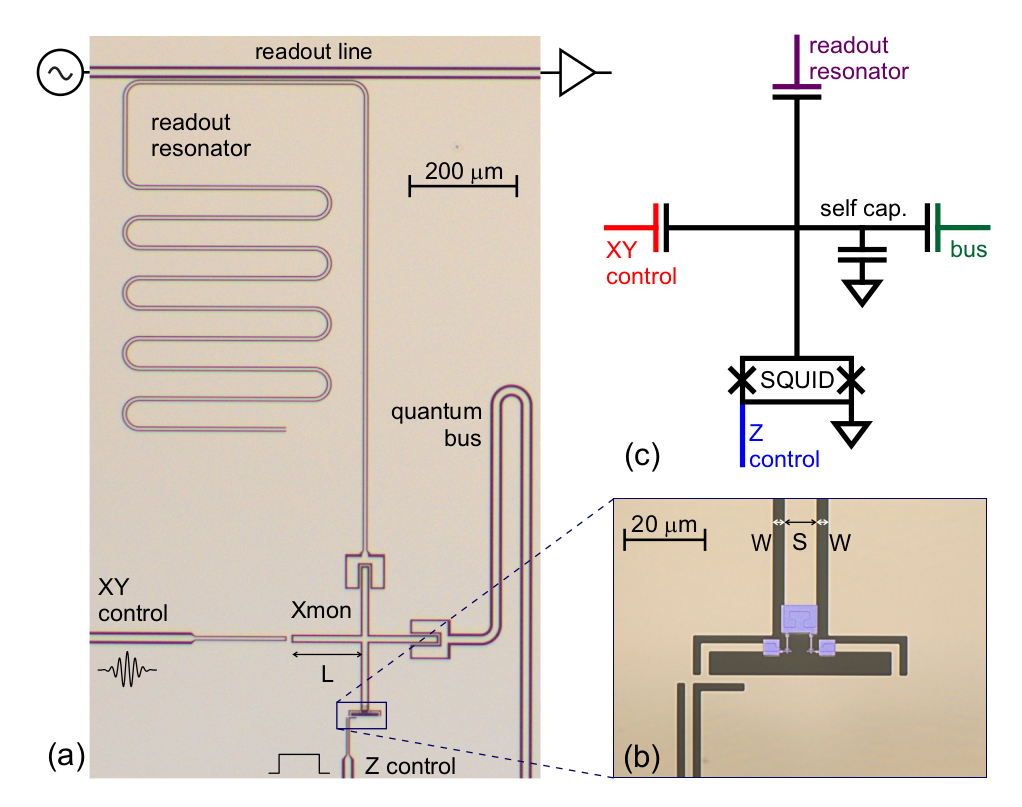
\includegraphics[width=\linewidth]{xmon.png}
  \caption{Original xmon qubit architecture now used in quantum computers at Google \cite{google}. Beige repersents the superconducting film (an uninterrupted ground plane) and dark grey repersents a gap of exposed crystalline substrate. The small beige lines between the pairs of dark exposed lines implement the center line of a continuous coplanar waveguide structure. The cross shaped capacitance is implemented in this coplanar structure, where each qubit shares the same grounding to the entire ground plane on chip. Images and illustration from \cite{xmon}.}
  \label{fig:xmon}
\end{figure}



\section{outlook}

From the past two decades of rapid progress, one lesson learned has been that the simplest limiting cases of qubits, the Cooper pair box and the flux qubit, each have their own advantages and disadvantages that presently cannot be engineered away entirely. The adoption of superconducting circuits whose dynamics depend more strongly on both charge and flux, such as the transmon, allowed a better compromised design for reproduceability and coherence times. Some new designs that lie closer to the spectrum of a true flux qubit, but with different physics, include fluxonium and the capacitively shunted flux qubit\citep{CSFQ}. Especially in the case of fluxonium, a different description is required, where the quantum information encoded is not solely a charge or flux eigenstate \cite{fluxoniumtheory}. This added complexity offers the possibility of avoiding the charge noise that degrades the CPB, while maintaining anharmoncity and reproduceability. As an example, a recent fluxonium qubit encased in a 3D cavity achieved coherence times well exceeding a microsecond \cite{fluxonium_quasiparticle} by the suppression of quasiparticle dissipation. We have also seen that theoretical understanding of noise, such as the TLS description of charge noise, has played a crucial role in improving coherence times so that quantum algorithms can be realized. A current example following this line of reasoning is the active effort to leverage spectroscopy to study non-Gaussian noise \cite{non_gaussian_noise} coupling to the system, for which there is currently not a complete description. It is not obvious if some insight leading to a new superconducting qubit paradigm or a more complete theoretical understanding of noise will be the next step for improving coherence consistently above a millisecond. Based on past experience, we can expect these two efforts to stay connected and to continue the discourse between theory and experiment.  



%\bibliographystyle{IEEEtranN}
%\bibliographystyle{aipnum4-1}
\bibliographystyle{unsrt}
\bibliography{Bib_SCQB}

\end{document}


